\subsection*{What turns detection into override}

The experiments above establish that agents relay plausible values and override impossible ones, and that a second field in the record moves the boundary. Four further registered experiments ask what, short of an external source, changes relay (Fig.~7; Supplementary Tables~1--5).

\textbf{Instructions remove relay only where the record contradicts the value.} We reran three cells under three prompt variants (Methods). On the chemistry agreement cell, where the formula and SMILES contradict the molecular weight, removing the instruction to use the provided tools lowered relay from 80--91\% to 34--51\% for Opus~5, Argon and Flash (paired McNemar, $p \le 4\times10^{-9}$), and telling the agent that the database contains errors and the formula is authoritative lowered it to 0--1\% in every model. On coherent protein errors, where nothing in the record contradicts the value, no instruction changed relay (92--100\% under every variant). The registered prediction that the tool instruction would matter by fewer than 10 points failed; the prediction that no instruction would reach coherent errors held.

\textbf{The output format decides whether memory is consulted.} A fourth variant asked for the database value and the agent's best estimate as separate fields. On coherent errors this variant lowered relay from 98\% to 52\% for Opus~5 and from 96\% to 0\% for Argon, with DeepSeek at 90\% (from 94\%). Nothing in the record could have produced these answers. The memory probe (below) shows that these models hold the current value for most proteins, and separating the estimate from the record let that memory be used. The format did not give a reliable audit trail, however: the stated database value matched the record in only 0--28\% of runs on the protein cell and 63--100\% on the chemistry cell (Methods).

\textbf{Agreement is the absence of contradiction, not a count of agreeing fields.} In the repetition experiment, a verbatim copy of the corrupted weight in a second field lowered relay rather than raising it (pooled 68\% to 52\%, two-sided McNemar $p < 10^{-10}$; lower in every model, significantly in three), a derived field that agreed raised it by 2--7 points, and a copy that disagreed removed it almost entirely (0--3\%). The registered prediction that repetition would act as agreement failed. What the agent responds to is a disagreement inside the record; agreement from a derived field adds only modestly to the weight alone.

\textbf{Memory is a tie-breaker, not the cause of relay.} Asked without tools for the length of each protein in the historical set, the three models gave the superseded value for 8--9\% of proteins and the current value for 61--67\%. Without a second source, proteins for which memory held the current value were still relayed at 91--100\%: the record won over a correct memory. With the labelled second source present, proteins whose memory held the superseded value were relayed far more often (Opus~5, 13/21 versus 2/144, $p < 10^{-10}$; DeepSeek, 17/18 versus 38/150, $p = 1 \times 10^{-8}$), so when the record shows a conflict, memory decides it.

\textbf{Withholding the field removes relay entirely.} A harness that drops any derivable field failing its check, with no note, left 0 of 709 corrupted numeric fields relayed across three models, two domains and both conditions, at the cost of 8 wrong answers in 200 DeepSeek protein runs. Identifier fields, which the check does not cover, were still relayed (0--8\% of protein runs, 4--48\% of compound-name runs).

\begin{figure}[p]
\centering
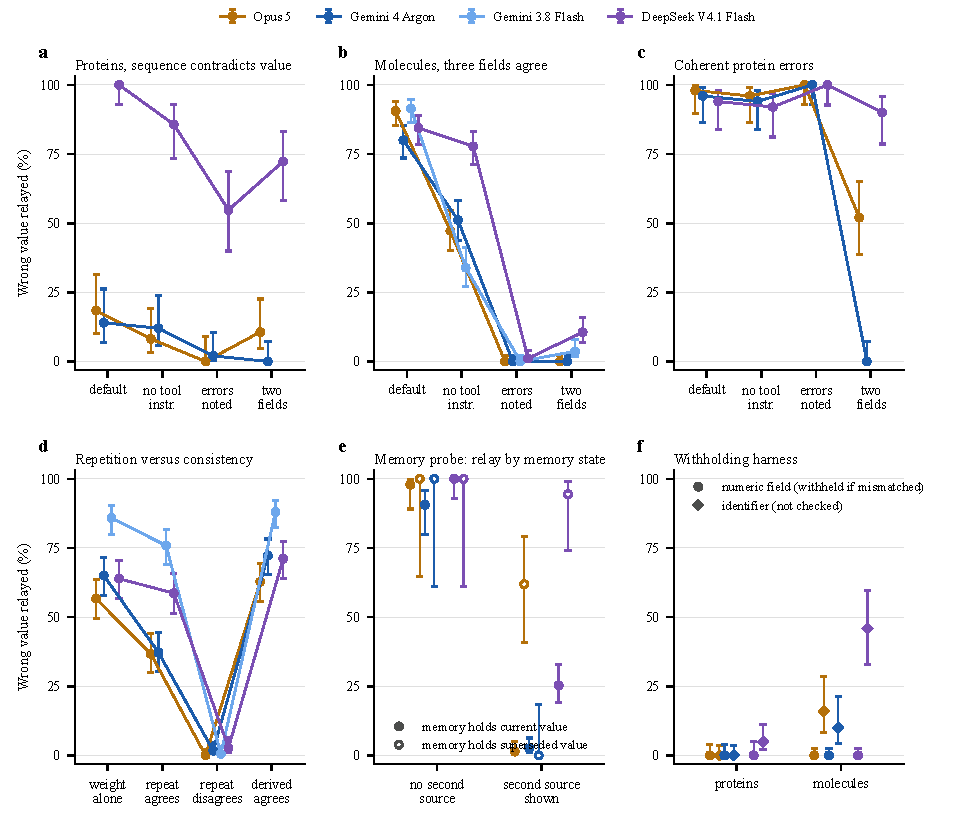
\includegraphics[width=\linewidth]{../figures/nmi_mechanism.pdf}
\caption{\textbf{What turns detection into override.} \textbf{a--c}, Relay under four system prompts: the registered default; without the instruction to use the tools (no tool instr.); with a note that the database contains errors and the sequence or formula is authoritative (errors noted); with the answer and the record's value asked for as separate fields (two fields) on three cells: protein tasks whose full record contradicts the value (\textbf{a}), the chemistry agreement cell with three fields agreeing with the wrong weight, three samples (\textbf{b}), and coherent protein errors that nothing in the record contradicts (\textbf{c}). \textbf{d}, Repetition versus consistency: relay of a wrong molecular weight alone, with a verbatim repeat that agrees, with a repeat that disagrees, and with a derived field (heavy-atom count) that agrees; 60 compounds, three samples. \textbf{e}, Memory probe: relay of the superseded value for proteins whose memory held the current (filled) or the superseded (open) length, without a second source (full record) and with the second source shown (three samples). \textbf{f}, Withholding harness: relay of corrupted numeric fields, withheld when they fail the derivation check (circles), and of identifiers, which the harness does not check (diamonds); impossible and plausible pooled. Markers give relay with 95\% Wilson intervals; lines connect one model.}
\label{fig:mechanism}
\end{figure}
